%%%%%%%%%%%%%%%%%%%%%%%%%%%%%%%%%%%%%%%%%
% Friggeri Resume/CV
% XeLaTeX Template
% Version 1.1 (9/2/15)
%
% This template has been downloaded from:
% http://www.LaTeXTemplates.com
%
% Original author:
% Adrien Friggeri (adrien@friggeri.net)
% https://github.com/afriggeri/CV
%
% License:
% CC BY-NC-SA 3.0 (http://creativecommons.org/licenses/by-nc-sa/3.0/)
%
% Important notes:
% This template needs to be compiled with XeLaTeX and the bibliography, if used,
% needs to be compiled with biber rather than bibtex.
%
%%%%%%%%%%%%%%%%%%%%%%%%%%%%%%%%%%%%%%%%%
\documentclass[]{../friggeri-cv} % Add 'print' as an option into the square bracket to remove colors from this template for printing
\usepackage[danish]{babel}
\usepackage{icomma}
%\addbibresource{bibliography.bib} % Specify the bibliography file to include publications

\begin{document}

\header{morten}{schiøler}{consultant@Deloitte Consulting, Business System Transformation} % Your name and current job title/field

%----------------------------------------------------------------------------------------
%	SIDEBAR SECTION
%----------------------------------------------------------------------------------------

\begin{aside} % In the aside, each new line forces a line break
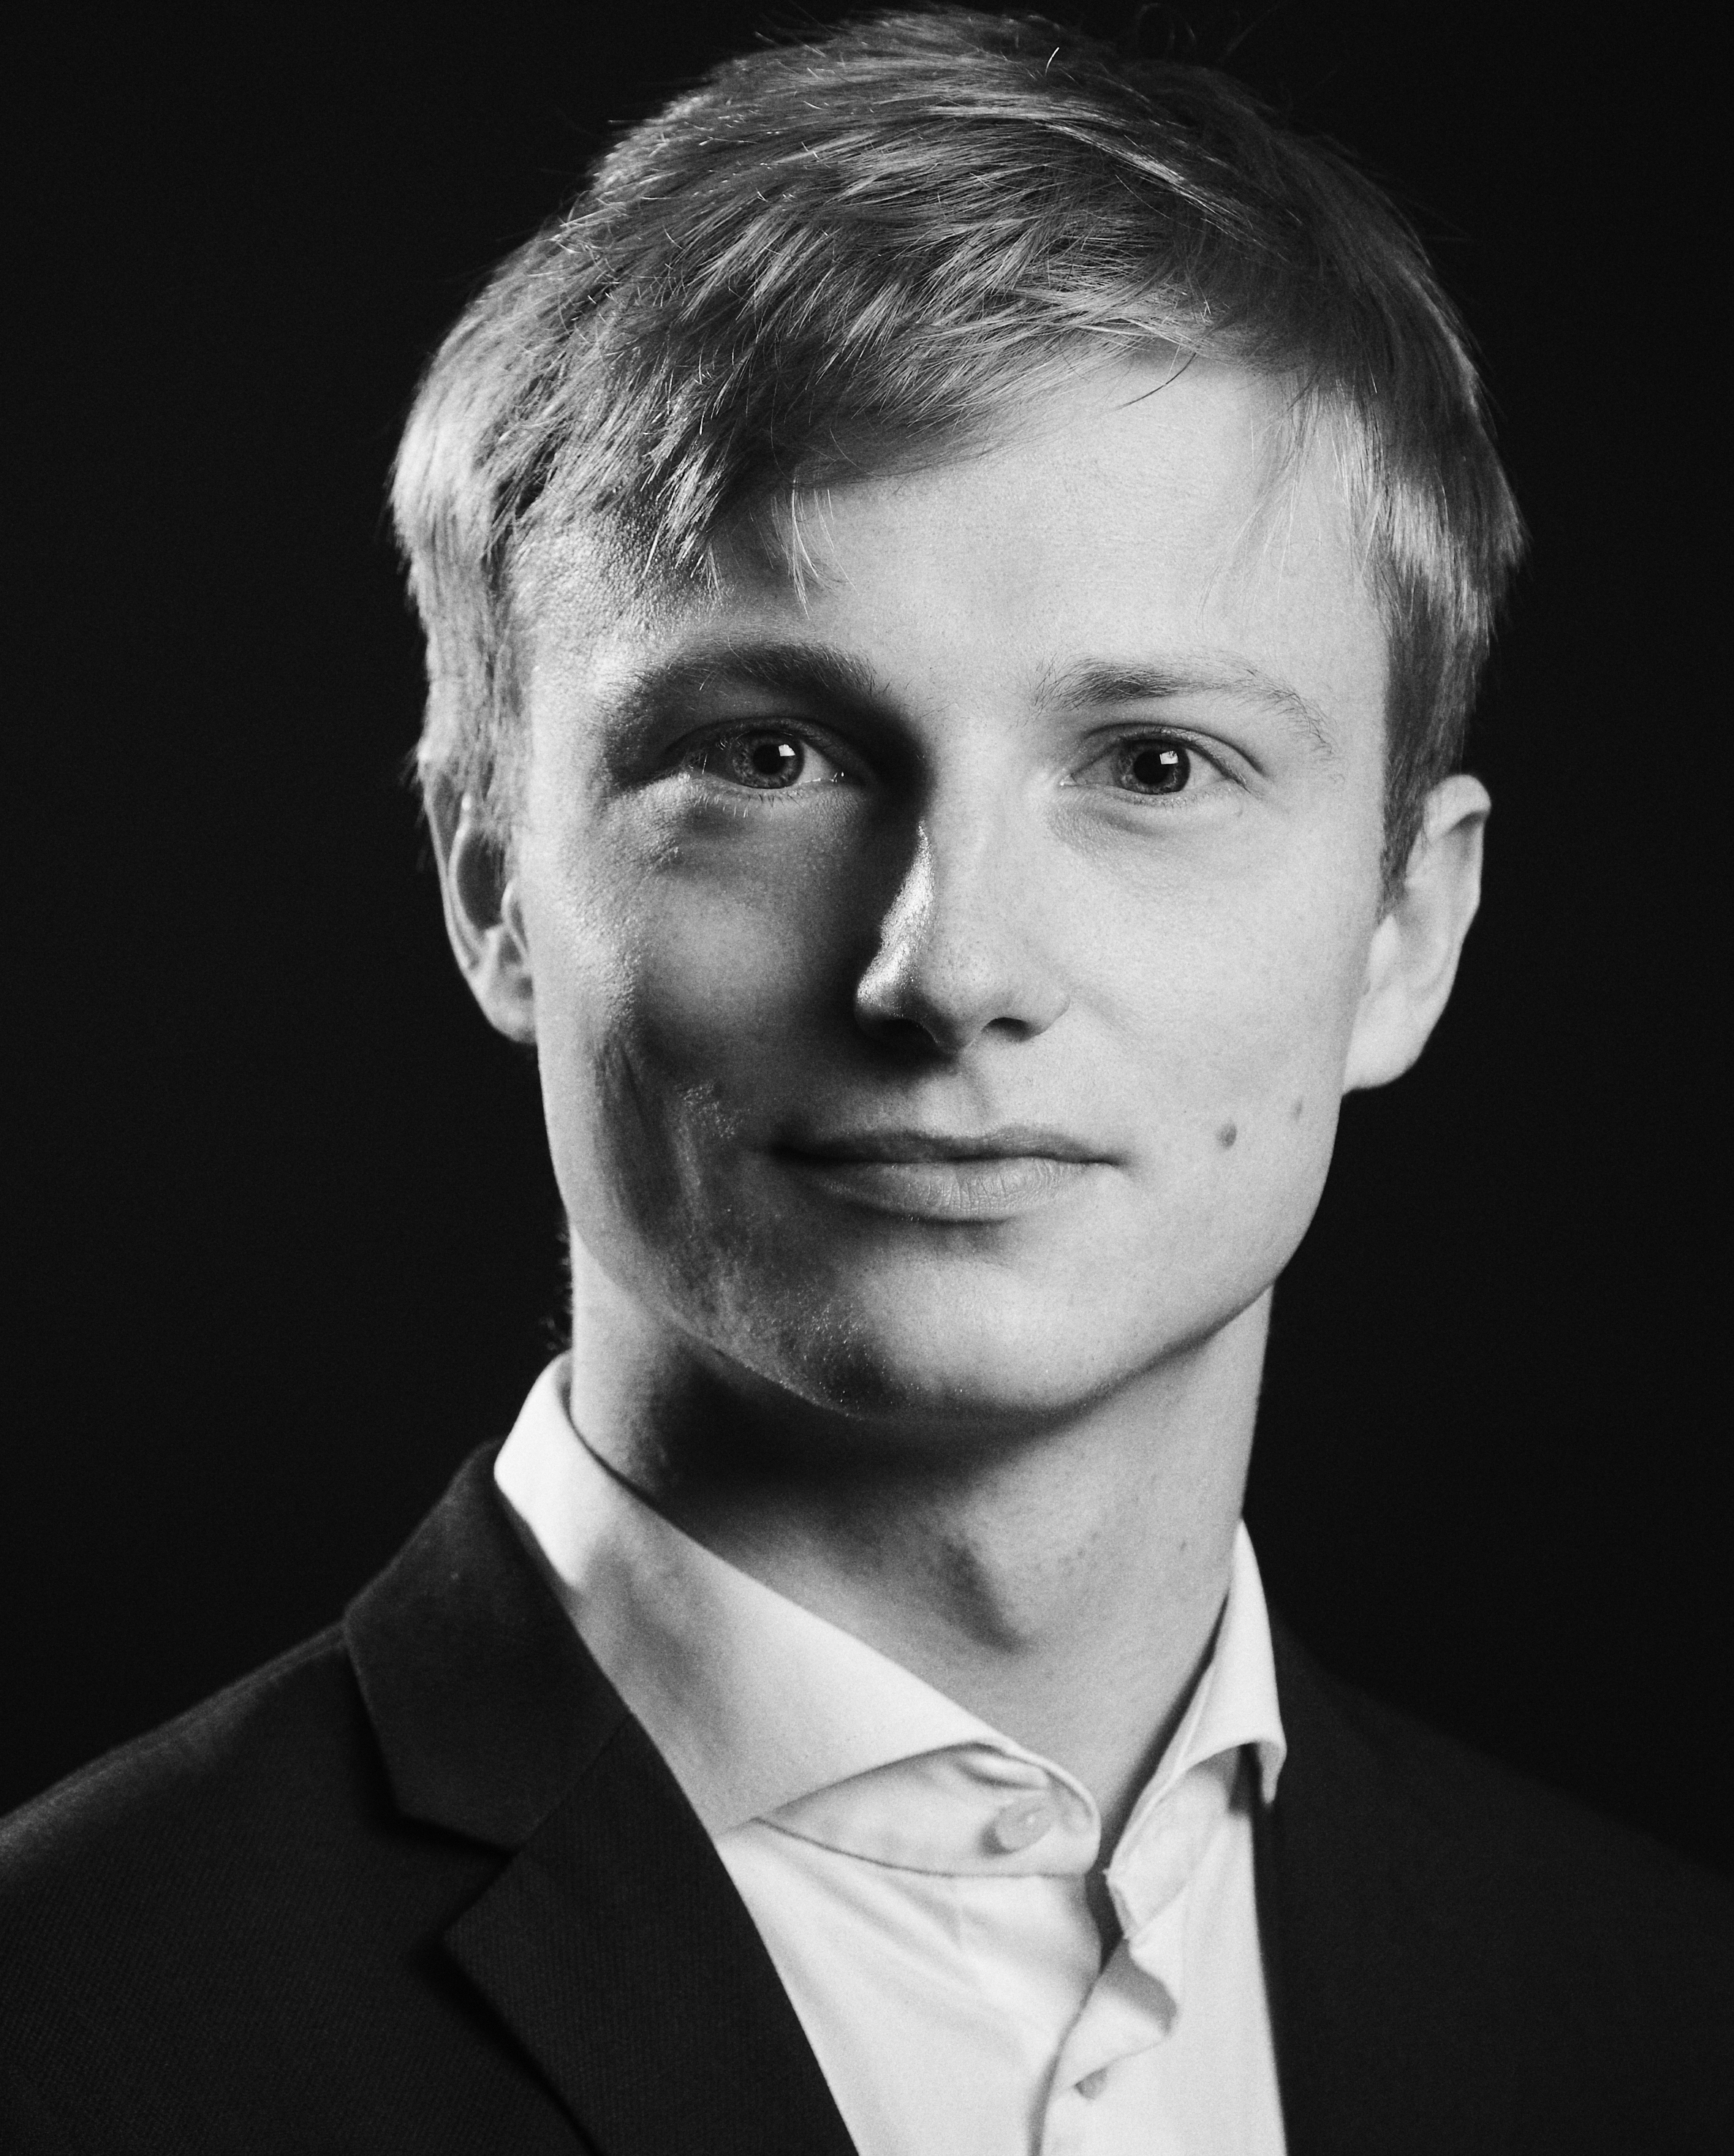
\includegraphics[width=\linewidth]{../graphics/pic8x10.jpg}
\section{kontakt}
Guldborgvej 5, st.th
2660 Brøndby Strand
~
+45 30 93 43 16
{\small \href{mailto:mortenschioler@gmail.com}{mortenschioler@gmail.com}}
\section{sprogkundskaber}
	dansk:  \quad modersmål
	engelsk: \quad flydende
	fransk: \quad begrænset praktisk færdighed
%norwegian and swedish
\section{programmering}
Java, SAS, SQL,
\textsc{MATLAB}, Python, CPLEX,
R Statistics
%{\color{red} $\varheartsuit$} \LaTeX 
\end{aside}

%----------------------------------------------------------------------------------------
%	EDUCATION SECTION
%----------------------------------------------------------------------------------------

\section{profil}
En dreven og talentfuld dimmitend fra DTU. Jeg ser mig selv i en stilling i en rådgivende konsulentvirksomhed på grund af  min forkærlighed for den omskiftelige arbejdsplads, samt evne til hurtigt og effektivt at tilegne mig erfaring, forstå  nye metoder og anvende dem  i kreativ problemløsning. Jeg udmærker mig desuden ved  at bidrage til at drive retningen af de projekter jeg medvirker i, og til at motivere og lytte til mine holdkammerater   uden at begrænse dem.

\section{uddannelse}
\begin{entrylist}
%------------------------------------------------
\entry
{2014--2016}
{Kandidat {\normalfont i Transport og Logistik}}
{Danmarks Tekniske Universitet, Kgs. Lyngby}
{Omfattende studier i matematisk modellering, planlægning samt operationsanalyse, CBA og risikoanalyse. Tog kurser som f.eks. Heltalsprogrammering, Netværksoptimering og Risk Management. Publicerede videnskabelig artikel  som medforfatter på baggrund af speciale om parameterestimation i ny rutevalgsmodel. Afsluttet med et 12-tal (gennemsnit 11.25).
}


\entry
{2011--2014}
{Bachelor {\normalfont i Produktion og Konstruktion}}
{Danmarks Tekniske Universitet, Kgs. Lyngby}
{Bredt fagområde, bl.a. avanceret matematik og operationsanalyse, statistik og sandsynlighedsregning. Derudover fysik, styrkelære, procesteknik mv. Konkurrerede i Racing Aeolus  i Holland, 2014, for winDTUrbine. Konstruerede køretøj, der drives af modvind; køretøjet er nu international rekordholder ved at bevæge sig 101.8 \% af vindens hastighed.}
%------------------------------------------------
%------------------------------------------------

\end{entrylist}

%----------------------------------------------------------------------------------------
%	WORK EXPERIENCE SECTION
%----------------------------------------------------------------------------------------

\section{erfaring}
\begin{entrylist}
%------------------------------------------------
\entry
{2016--}
{DTU Management, Transport DTU}
{Danmarks Tekniske Universitet, Kgs. Lyngby}
{Videnskabelig assistent hos institut for Management. Adskillige opgaver, involverende modeludvikling, programmering, dataanalyse og grundforskning.}

\entry
{2015}
{DTU Management Engineering}
{Danmarks Tekniske Universitet, Kgs. Lyngby}
{Hjælpelærer i Heltalsprogrammering for kandidatstuderende efter umotiveret ansøgning. Modtog  skriftlig anbefaling.}

\entry
{2013--2015}
{DTU Fysik}
{Danmarks Tekniske Universitet, Kgs. Lyngby}
{Hjælpelærer i Fysik 1, kursus 10020. Opnåede  respekt og sympati blandt både elever og kollegaer.}

\entry
{2014}
{DTU Management Engineering}
{Danmarks Tekniske Universitet, Kgs. Lyngby}
{Hjælpelærer i Introduktion til Operationsanalyse, kursus 42101.}

\entry
{2011--2015}
{KAB {\normalfont Københavns Almennyttige Boligsselskab}}
{Nybrogård Kollegiets Klagenævn}
{Ugentligt arbejde med behandling af interne klagesager på kollegiet.
}
%------------------------------------------------
\end{entrylist}


%----------------------------------------------------------------------------------------
%	COMMUNICATION SKILLS SECTION
%----------------------------------------------------------------------------------------
%\section{kvalifikationer}
%\begin{entrylist}
%%------------------------------------------------
%\entry
%{2011--2014}
%{Udvalgte bachelorkurser}
%{DTU}
%{videregående matematik 1 og 2, statistik, sandsynlighedsregning, stokastisk simulation, programmering i Matlab, reguleringsteknik, operationsanalyse}
%\entry
%{2014--}
%{Udvalgte masterkurser}
%{DTU}
%{tidsrækkeanalyse (videregående statistik), multivariat statistik, risikomanagement, GIS og vejtrafikplanlægning,  heltalsprogrammering, netværksoptimering, introduktion til planlægning, planlægningsteori, TEMPOP (transport, økonomi, ledelse, planlægning, organisation og politik), transportmodeller, Avancerede transportmodeller, diskrete valgmodeller, intelligente transportsystemer (ITS),}
%%------------------------------------------------
%%------------------------------------------------
%\end{entrylist}

%----------------------------------------------------------------------------------------
%	AWARDS SECTION
%----------------------------------------------------------------------------------------

%\section{priser}
%\begin{entrylist}
%	%------------------------------------------------
%	%------------------------------------------------
%	\entry
%	{2010}
%	{Diplom for udmærkelse}
%	{Maribo Gymnasium, STX}
%	{For fremragende besvarelse i anden runde af den nationale Georg Mohr-konkurrence i matematik.}
%	%--------
%	\entry
%	{2011}
%	{Studentereksamen}
%	{Maribo Gymnasium, STX}
%	{Højeste gennemsnit på årgangen, 11,9$\times$1,03 = 12,3.}
%\end{entrylist}
%----------------------------------------------------------------------------------------
%	INTERESTS SECTION
%----------------------------------------------------------------------------------------
\section{interesser}
\textbf{professionelt:} matematisk modellering, programmering,  operationsanalyse,  fysik
\textbf{personligt:} klaver, guitar, kaffe, sprog, spil
%----------------------------------------------------------------------------------------
%	PUBLICATIONS SECTION
%----------------------------------------------------------------------------------------

%\section{publications}
%
%\printbibsection{article}{article in peer-reviewed journal} % Print all articles from the bibliography
%
%\printbibsection{book}{books} % Print all books from the bibliography
%
%\begin{refsection} % This is a custom heading for those references marked as "inproceedings" but not containing "keyword=france"
%\nocite{*}
%\printbibliography[sorting=chronological, type=inproceedings, title={international peer-reviewed conferences/proceedings}, notkeyword={france}, heading=subbibliography]
%\end{refsection}
%
%\begin{refsection} % This is a custom heading for those references marked as "inproceedings" and containing "keyword=france"
%\nocite{*}
%\printbibliography[sorting=chronological, type=inproceedings, title={local peer-reviewed conferences/proceedings}, keyword={france}, heading=subbibliography]
%\end{refsection}
%
%\printbibsection{misc}{other publications} % Print all miscellaneous entries from the bibliography
%
%\printbibsection{report}{research reports} % Print all research reports from the bibliography

%----------------------------------------------------------------------------------------

\end{document}
